Since the goal is to identify where each balls is between every shot an approach for detecting changes on the table have to be made. These changes should be changes in ball positions and not if a hand or a que is present in the image.\\

\subsection{Detect occlusions:}
The first step is to detect weather or not parts of the table is occluded or not. This occlusion could be caused by human interaction or foreign object placed within the cloth of the table. Detection will be used before finding position of balls. If the table is detected to be occluded then there will be no detection of balls before the table is no longer occluded. This will bring down faulty detections caused by cue or foreign objects.\\

When the table is detected\ref{sec:table-locate}, a mask for the cloth is made. This mask is made from a contour which have many different properties such as area and perimeter. These properties can be used when identifying if occlusions are present. By comparing the current image mask together with the mask made in the calibration and finding the difference in area or perimeter, detection should be possible.\\

Occlusion area factor:
\begin{equation}
\gamma = \frac{Area_{current mask}}{Area_{calibrated mask}}
\label{eq:area}
\end{equation}

Occlusion perimeter factor:
\begin{equation}
\kappa = \frac{Perimeter_{current mask}}{Perimeter_{calibrated mask}}
\label{eq:perimeter}
\end{equation}

The two factors in \ref{eq:area} and \ref{eq:perimeter} will be found for various interference with the cloth.

\textbf{Without occlusions:}\\

\begin{figure}[H]
\centering
\subfloat[Cloth found in calibration.]
{
	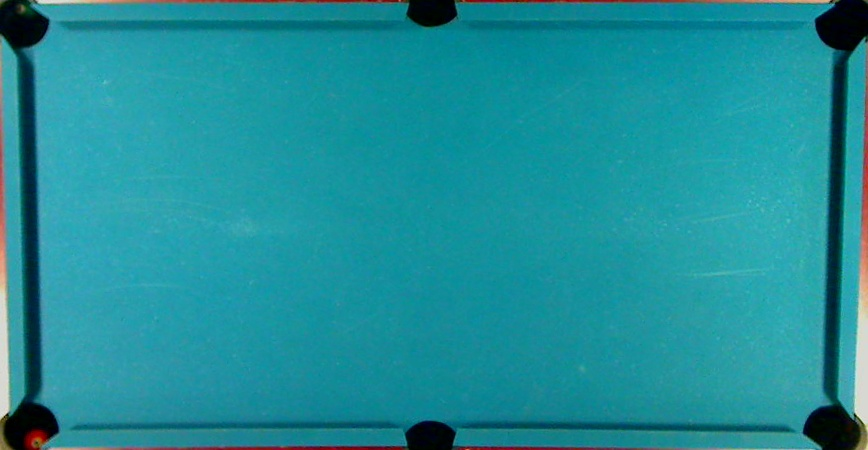
\includegraphics[width=0.3\textwidth]{images/occlutest/w_o_balls_}
}
\subfloat[Mask found in calibration.]
{
	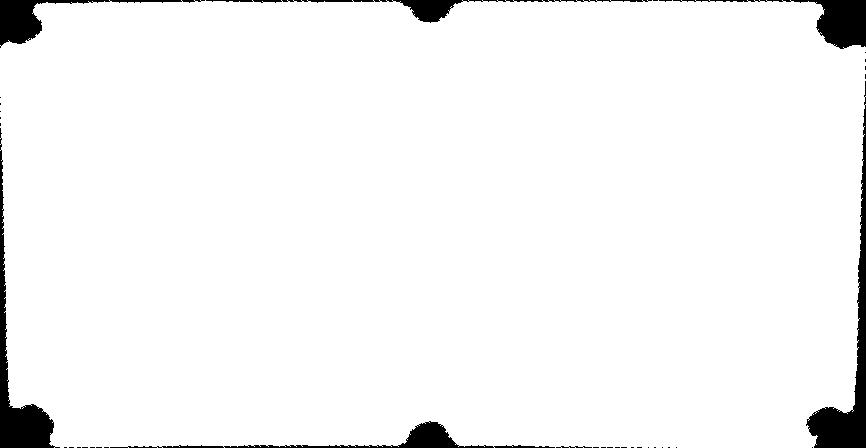
\includegraphics[width=0.3\textwidth]{images/occlutest/mask_calib}
}\\
\end{figure}

\textbf{Balls on table:}\\
\begin{figure}[H]
\centering
\subfloat[Balls on table.]
{
	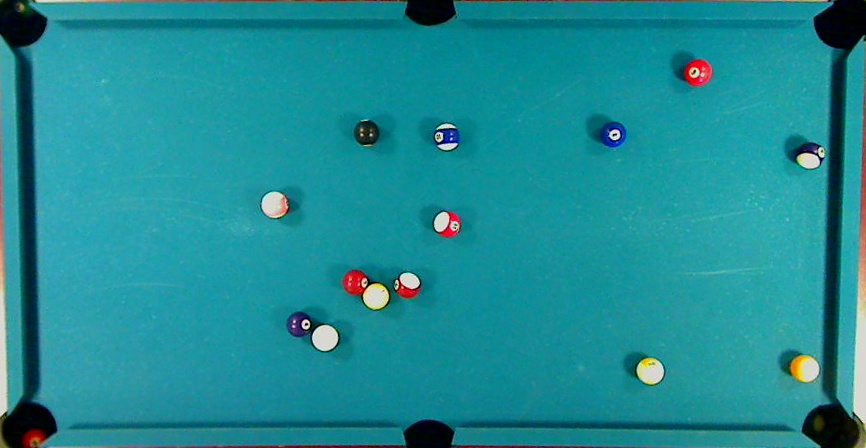
\includegraphics[width=0.3\textwidth]{images/occlutest/w_balls}
}
\subfloat[Mask found with balls on table.]
{
	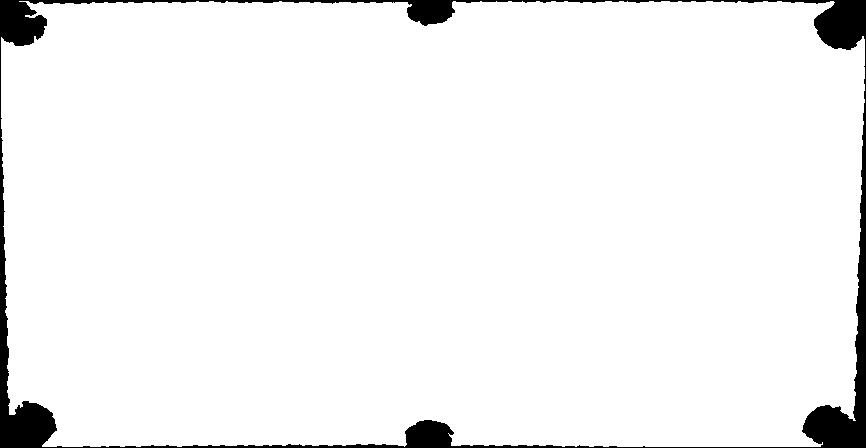
\includegraphics[width=0.3\textwidth]{images/occlutest/mask_w_balls}
}\\
\end{figure}

\textbf{Occluded by cue:}\\
\begin{figure}[H]
\centering
\subfloat[Cue occluding table.]
{
	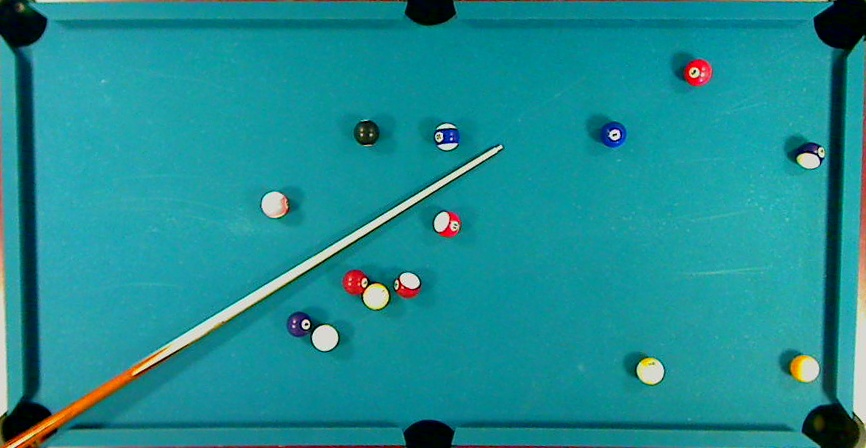
\includegraphics[width=0.3\textwidth]{images/occlutest/w_que}
}
\subfloat[Mask found with que occluding table.]
{
	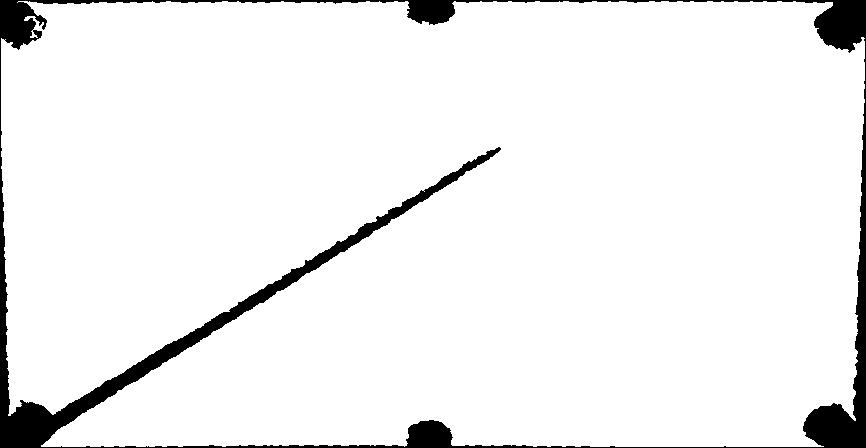
\includegraphics[width=0.3\textwidth]{images/occlutest/mask_w_que}
}\\
\end{figure}

\textbf{Occluded by person:}\\
\begin{figure}[H]
\centering
\subfloat[Person occluding table.]
{
	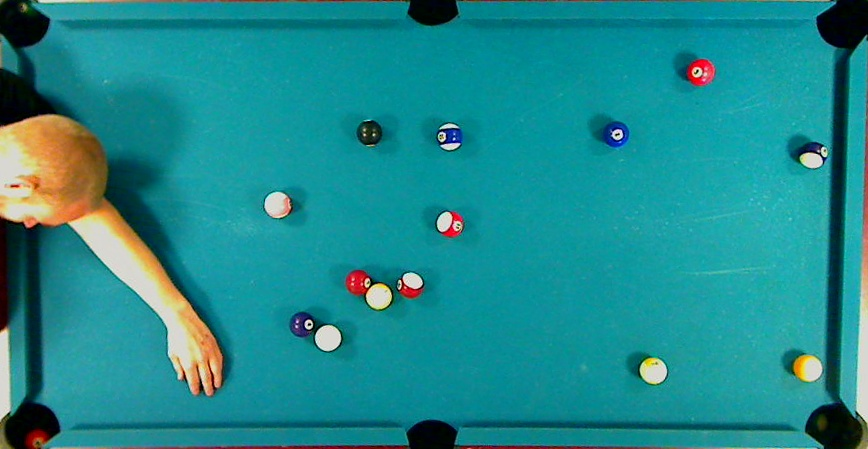
\includegraphics[width=0.3\textwidth]{images/occlutest/with_jesper}
}
\subfloat[Mask found with person occluding table.]
{
	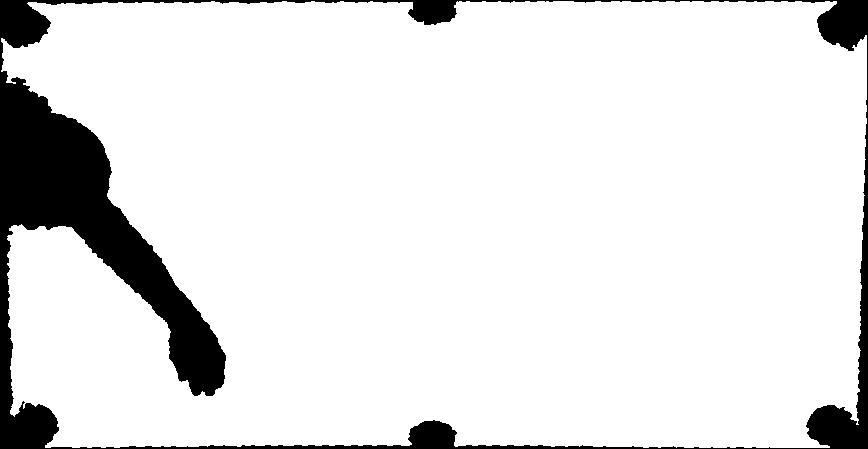
\includegraphics[width=0.3\textwidth]{images/occlutest/mask_with_jesper}
}\\
\end{figure}

\textbf{Occluded by chair:}\\
\begin{figure}[H]
\centering
\subfloat[Chair occluding table.]
{
	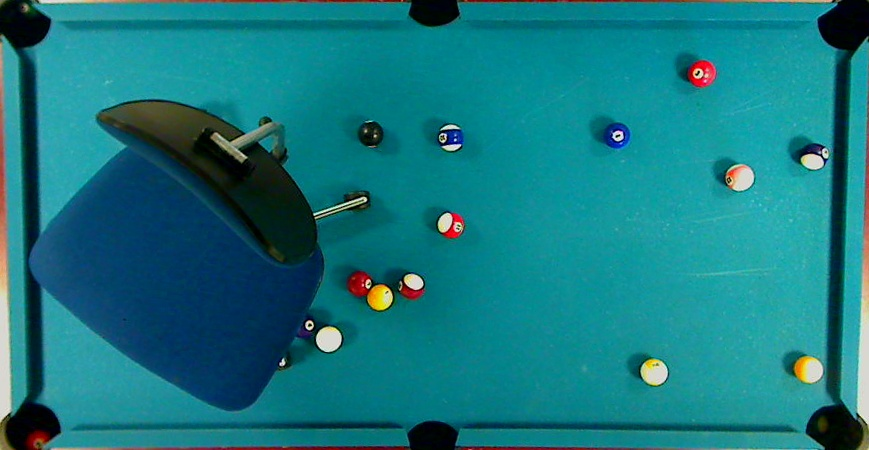
\includegraphics[width=0.3\textwidth]{images/occlutest/with_chair}
}
\subfloat[Mask found with chair occluding table.]
{
	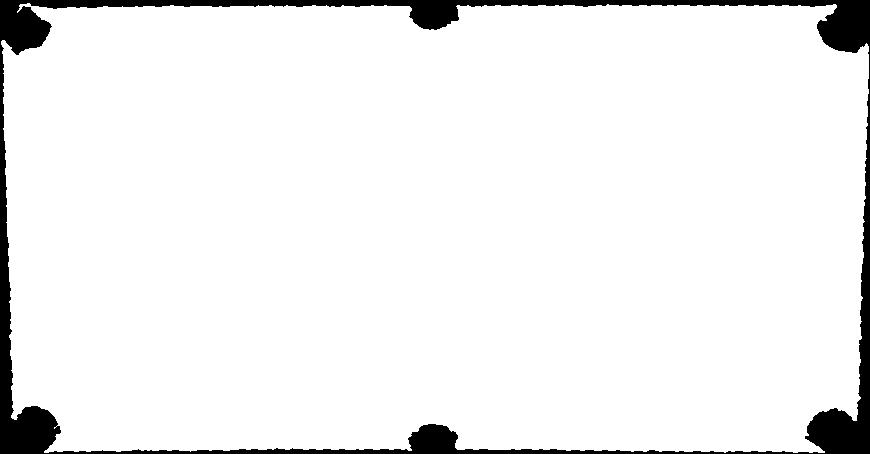
\includegraphics[width=0.3\textwidth]{images/occlutest/mask_w_chair}
}\\
\end{figure}

\textbf{Comparison of values and factors:}

\begin{figure}[H]
\centering
\begin{tabular}{|c|c|c|c|c|}
\hline  & Area & Perimeter & $\gamma$ & $\kappa$ \\ 
\hline Calibration & 371002 & 3597 & - & - \\ 
\hline Plain table & 369614 & 3212 & 0.996 & 0.89 \\
\hline Balls & 369647 & 3080 & 0.996 & 0.85  \\ 
\hline Cue & 364619 & 4134 & 0.983 & 1.15 \\ 
\hline Person & 348884 & 3796 & 0.940 & 1.06 \\ 
\hline Object & 370133 & 3092 & 0.997 & 0.86 \\ 
\hline 
\end{tabular} 
\end{figure}

\subsection{Detect movement of balls:}
After an occurred occlusion it is required to detect if movement of the balls is present. If there have been movement the balls would be found, identified and saved as one NAAAAAVN. If no movement is detected then the balls are expected to be in the same position which is already saved.\\

